\documentclass[xcolor=dvipsnames]{beamer}
\usepackage[T1]{fontenc}
\usepackage[utf8]{inputenc}
\usepackage[english,slovak]{babel}

\usepackage{amsmath}
\usepackage{amsthm}
\usetheme{Pittsburgh}
\useoutertheme{shadow}

\usepackage{graphicx}
\usepackage{caption}
\usepackage{subcaption}


\usepackage{listings}
\lstloadlanguages{Ruby}
\lstset{%
basicstyle=\ttfamily\color{black},
commentstyle = \ttfamily\color{red},
keywordstyle=\ttfamily\color{blue},
stringstyle=\color{orange}}



%-------------------------------------------------------------------------------------
\title{\bf Hybridný multirobotický systém}
\author{Michal CHOVANEC, Lukáš ČECHOVIČ \\Fakulta riadenia a informatiky}

\date[EURP]{\it Júl 2015}
\begin{document}

\begin{frame}
\titlepage
\end{frame}

%-------------------------------------------------------------------------------------
\begin{frame}{\bf Cieľ}

Problémy robotiky a umelej inteligencie

\begin{itemize}
	\item Manažérske
        \begin{itemize}
        \item Kto dá peniaze na násobenie matíc?
        \item Simuláciam sa "ľuďom" ťažko chápe
        \item Chcú vidieť priamy úžitok
        \end{itemize}

	\item Zmysluplné
        \begin{itemize}
        \item Reinforcement learning (Q-learning, SARSA)
        \item (Spiking) Neurónové siete
        \item Multirobotické systémy (mravce, roj)
        \item Strategické problémy (capture the flag, siege, prieskum)
        \item Robiť AI je cool
        \end{itemize}
\end{itemize}

\end{frame}


%-------------------------------------------------------------------------------------
\begin{frame}{\bf Kilobot}
\begin{columns}
	\begin{column}{0.48\textwidth}

	\begin{figure}[ht]
	\begin{center}
	\begin{minipage}{0.9\linewidth}
	\begin{center}
	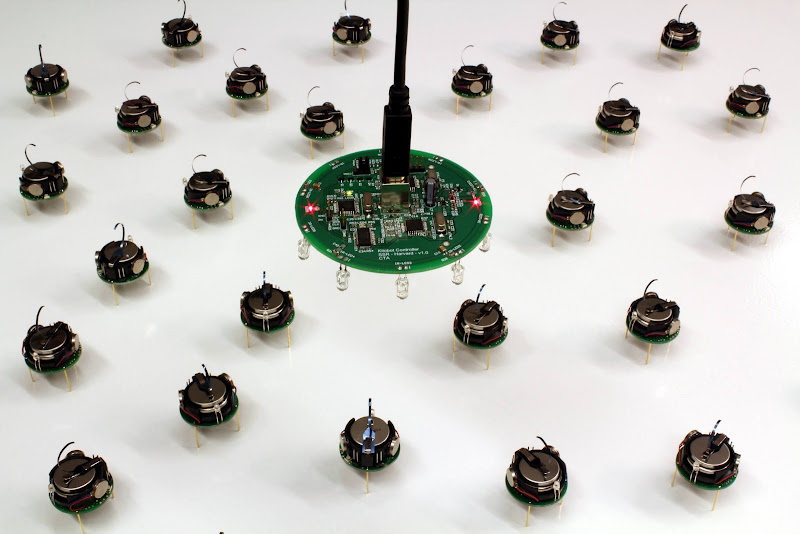
\includegraphics[width=1.0\textwidth]{images/kilobot.jpg}
	\end{center}
	\end{minipage}
	\end{center}
	\end{figure}

	\end{column}
	\begin{column}{0.48\textwidth}
		\begin{enumerate}
			\item Atmega328 16MHz, 8bit
            \item vibračné motory
			\item IR sensor, RGB LED
			\item senzor osvetlenia
            \item 33mm
		\end{enumerate}
	\end{column}
\end{columns}

\end{frame}


%-------------------------------------------------------------------------------------
\begin{frame}{\bf Formica}
\begin{columns}
	\begin{column}{0.48\textwidth}

	\begin{figure}[ht]
	\begin{center}
	\begin{minipage}{0.9\linewidth}
	\begin{center}
	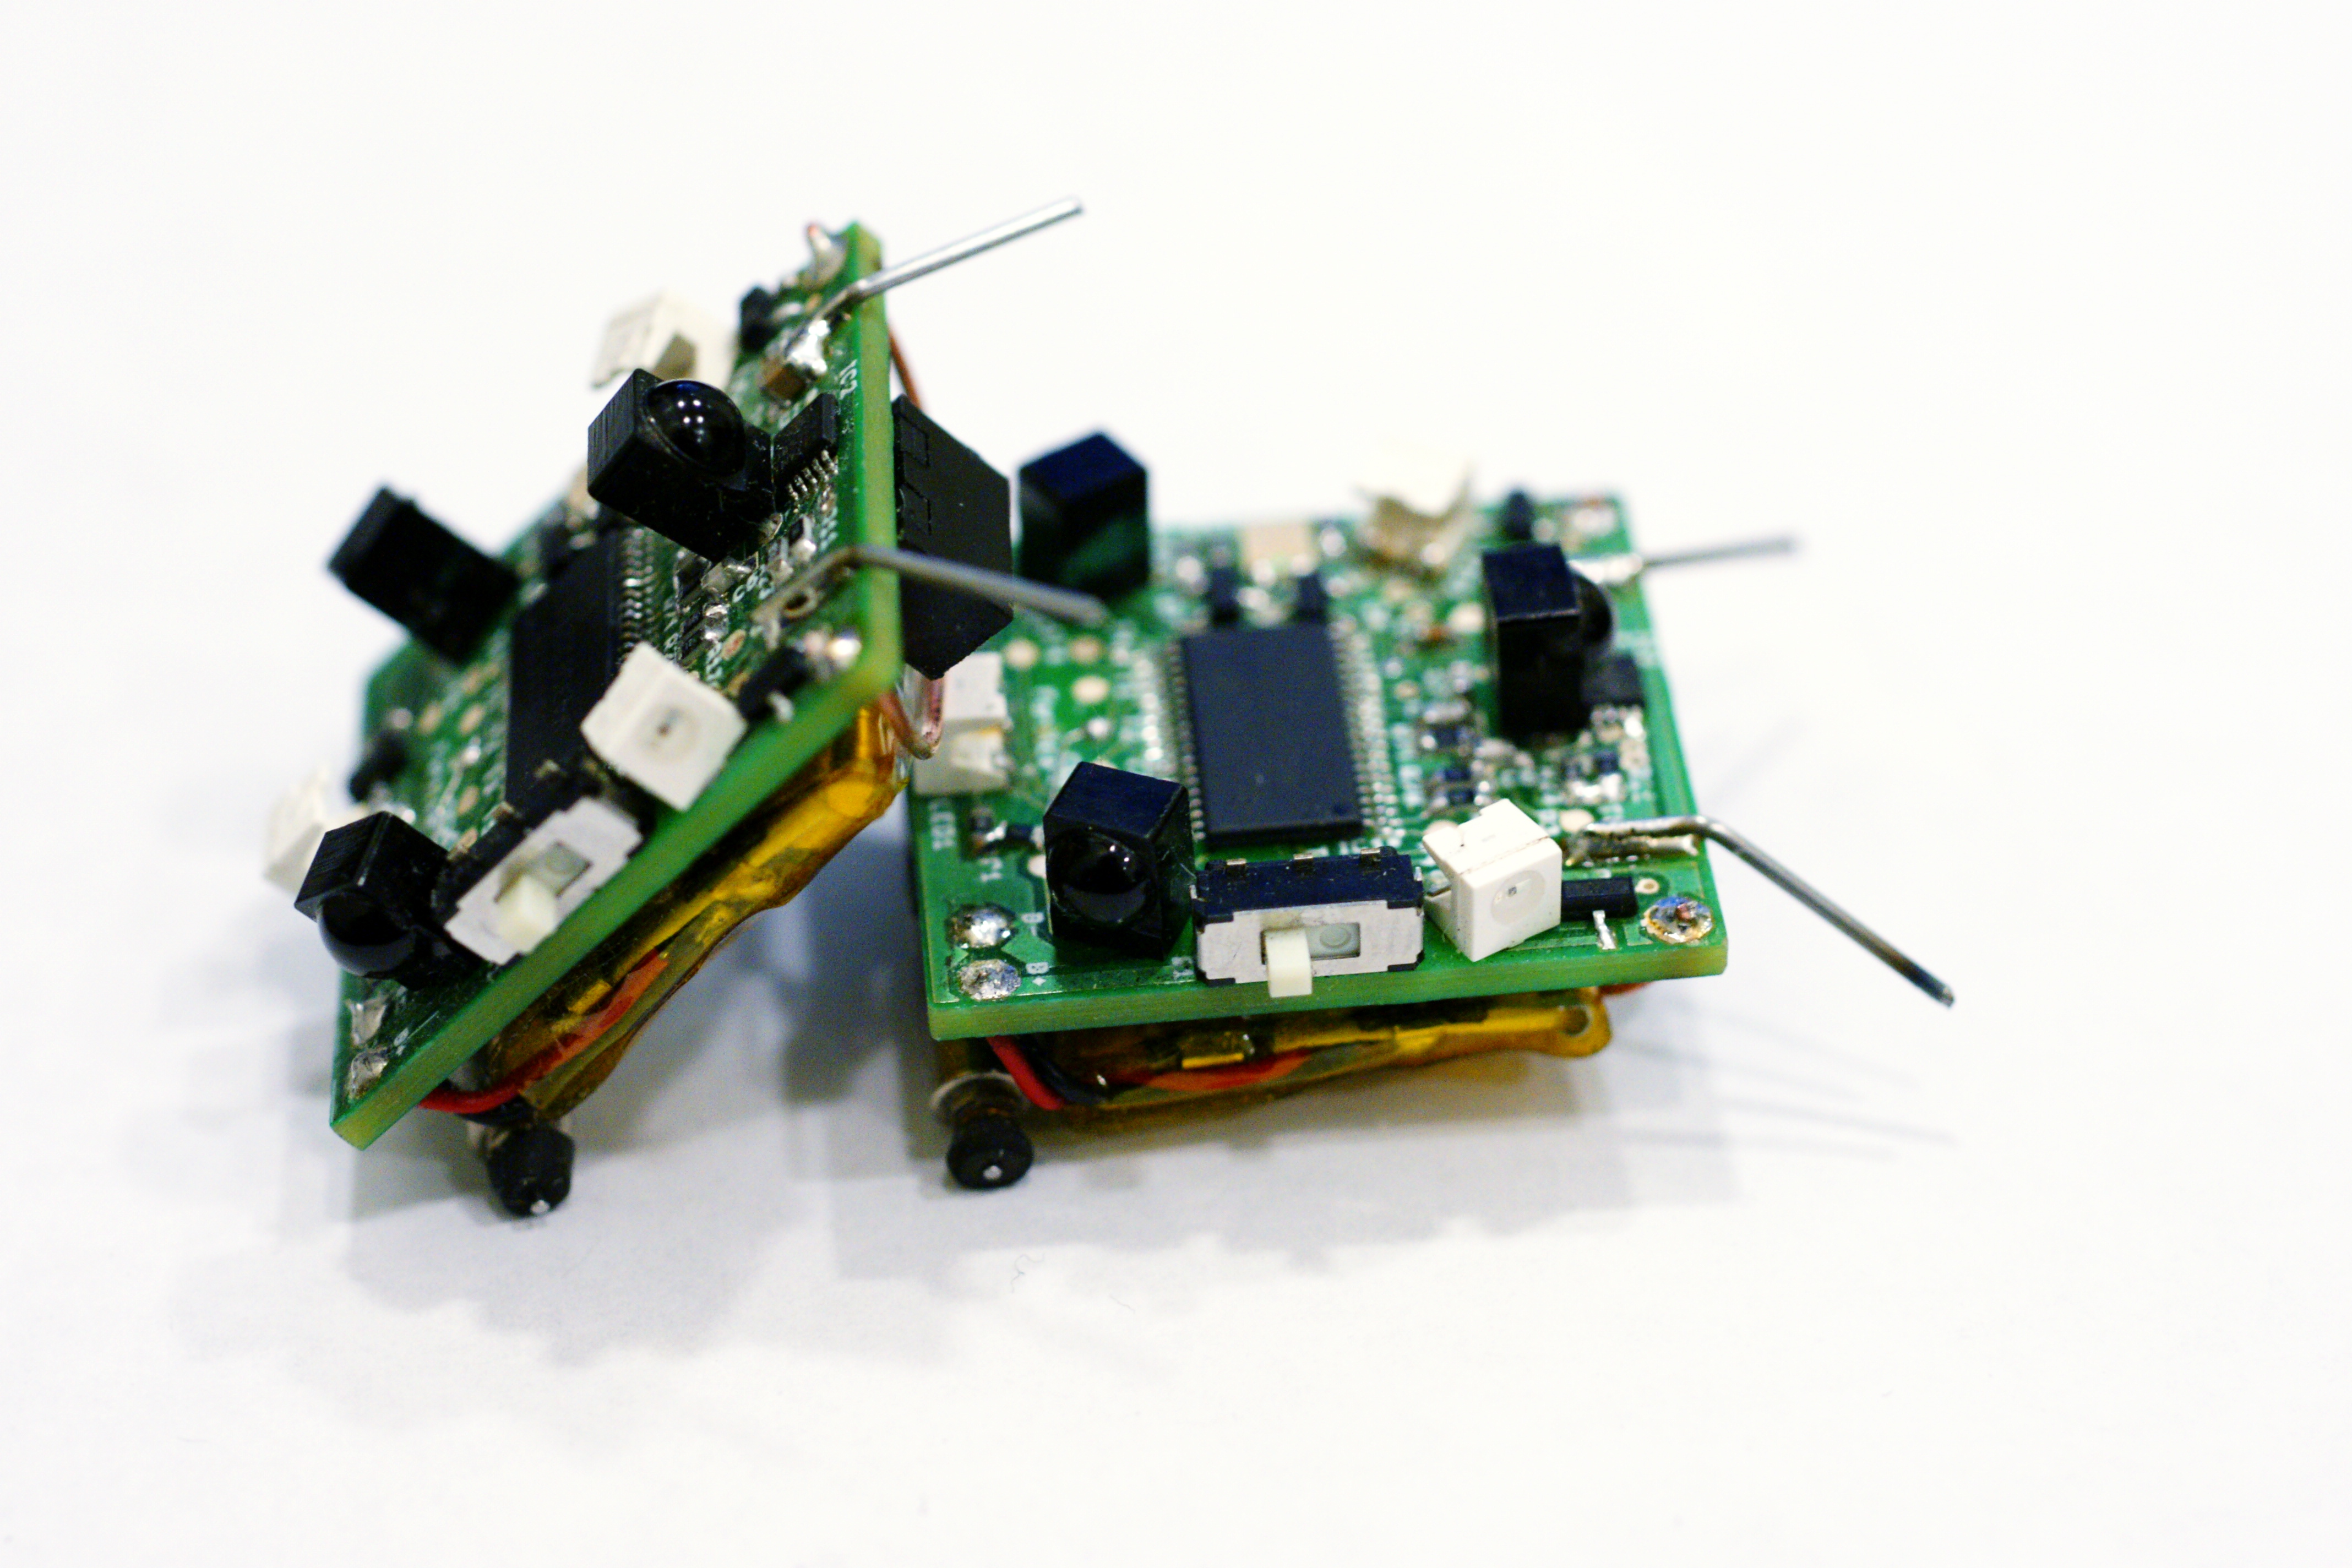
\includegraphics[width=1.0\textwidth]{images/formica.jpg}
	\end{center}
	\end{minipage}
	\end{center}
	\end{figure}

	\end{column}
	\begin{column}{0.48\textwidth}
		\begin{enumerate}
			\item MSP430F2234, 16MHz, 16bit
            \item mikromotory bez prevodu, kolesá
			\item 3x IR sensor
            \item 1x odrazový senzor
            \item 2x LED
            \item 30mm
		\end{enumerate}
	\end{column}
\end{columns}

\end{frame}




%-------------------------------------------------------------------------------------
\begin{frame}{\bf Khepera}
\begin{columns}
	\begin{column}{0.48\textwidth}

	\begin{figure}[ht]
	\begin{center}
	\begin{minipage}{0.9\linewidth}
	\begin{center}
	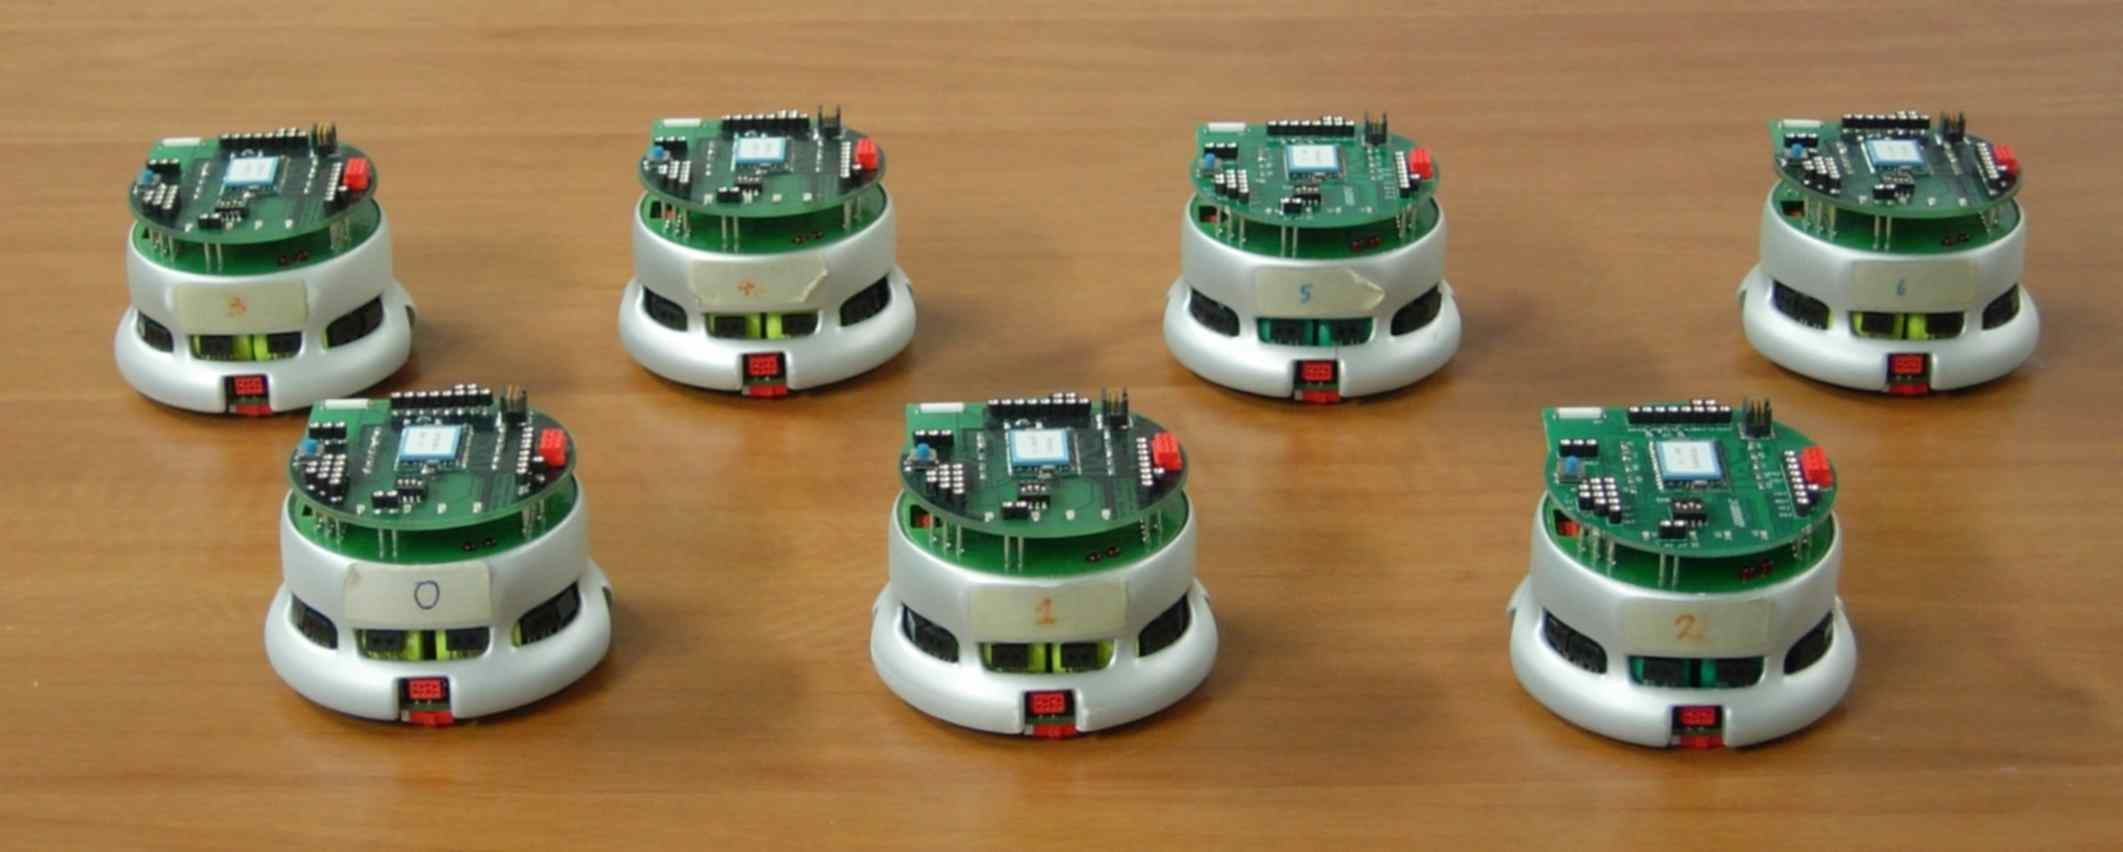
\includegraphics[width=1.0\textwidth]{images/khepera.jpg}
	\end{center}
	\end{minipage}
	\end{center}
	\end{figure}

	\end{column}
	\begin{column}{0.48\textwidth}
		\begin{enumerate}
			\item Motorola 68331, 25MHz, 32 bit
            \item mikromotory s prevodom, kolesá
			\item 8x IR sensor
            \item sensor osvetlenia
            \item sensor napájania
            \item LED
            \item 70mm
		\end{enumerate}
	\end{column}
\end{columns}

\end{frame}


%-------------------------------------------------------------------------------------
\begin{frame}{\bf Foot-bot}
\begin{columns}
	\begin{column}{0.48\textwidth}

	\begin{figure}[ht]
	\begin{center}
	\begin{minipage}{0.9\linewidth}
	\begin{center}
	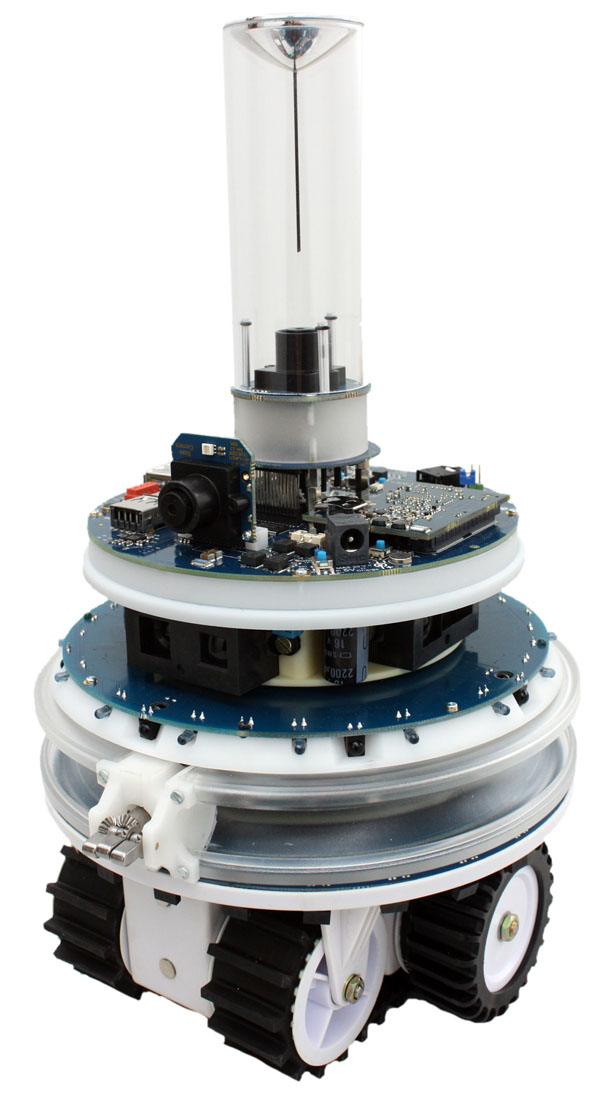
\includegraphics[width=0.9\textwidth]{images/foot_bot.jpg}
	\end{center}
	\end{minipage}
	\end{center}
	\end{figure}

	\end{column}
	\begin{column}{0.48\textwidth}
		\begin{enumerate}
            \item Linux 2.6, aseba
            \item 24xsenzory vzialenosti
            \item akcelerometer, magnetometer, gyroskop
            \item 2x mikrofón
			\item RFID
            \item kamera
            \item 170mm
		\end{enumerate}
	\end{column}
\end{columns}

\end{frame}


%-------------------------------------------------------------------------------------
\begin{frame}{\bf Cieľ}

Na čom sa teda pracuje :
\\
,,Ja by som to chcel na optickom princípe, žiadna magnetická doska'' \\
... \\
,,Zoberme najvačší LCD monitor, dajme to na ležato a roboti budú po ňom behať'' \\
\end{frame}

%-------------------------------------------------------------------------------------
\begin{frame}{\bf Súčasný stav projektu}

\begin{figure}[ht]
\begin{center}
\begin{minipage}{0.8\linewidth}
\begin{center}
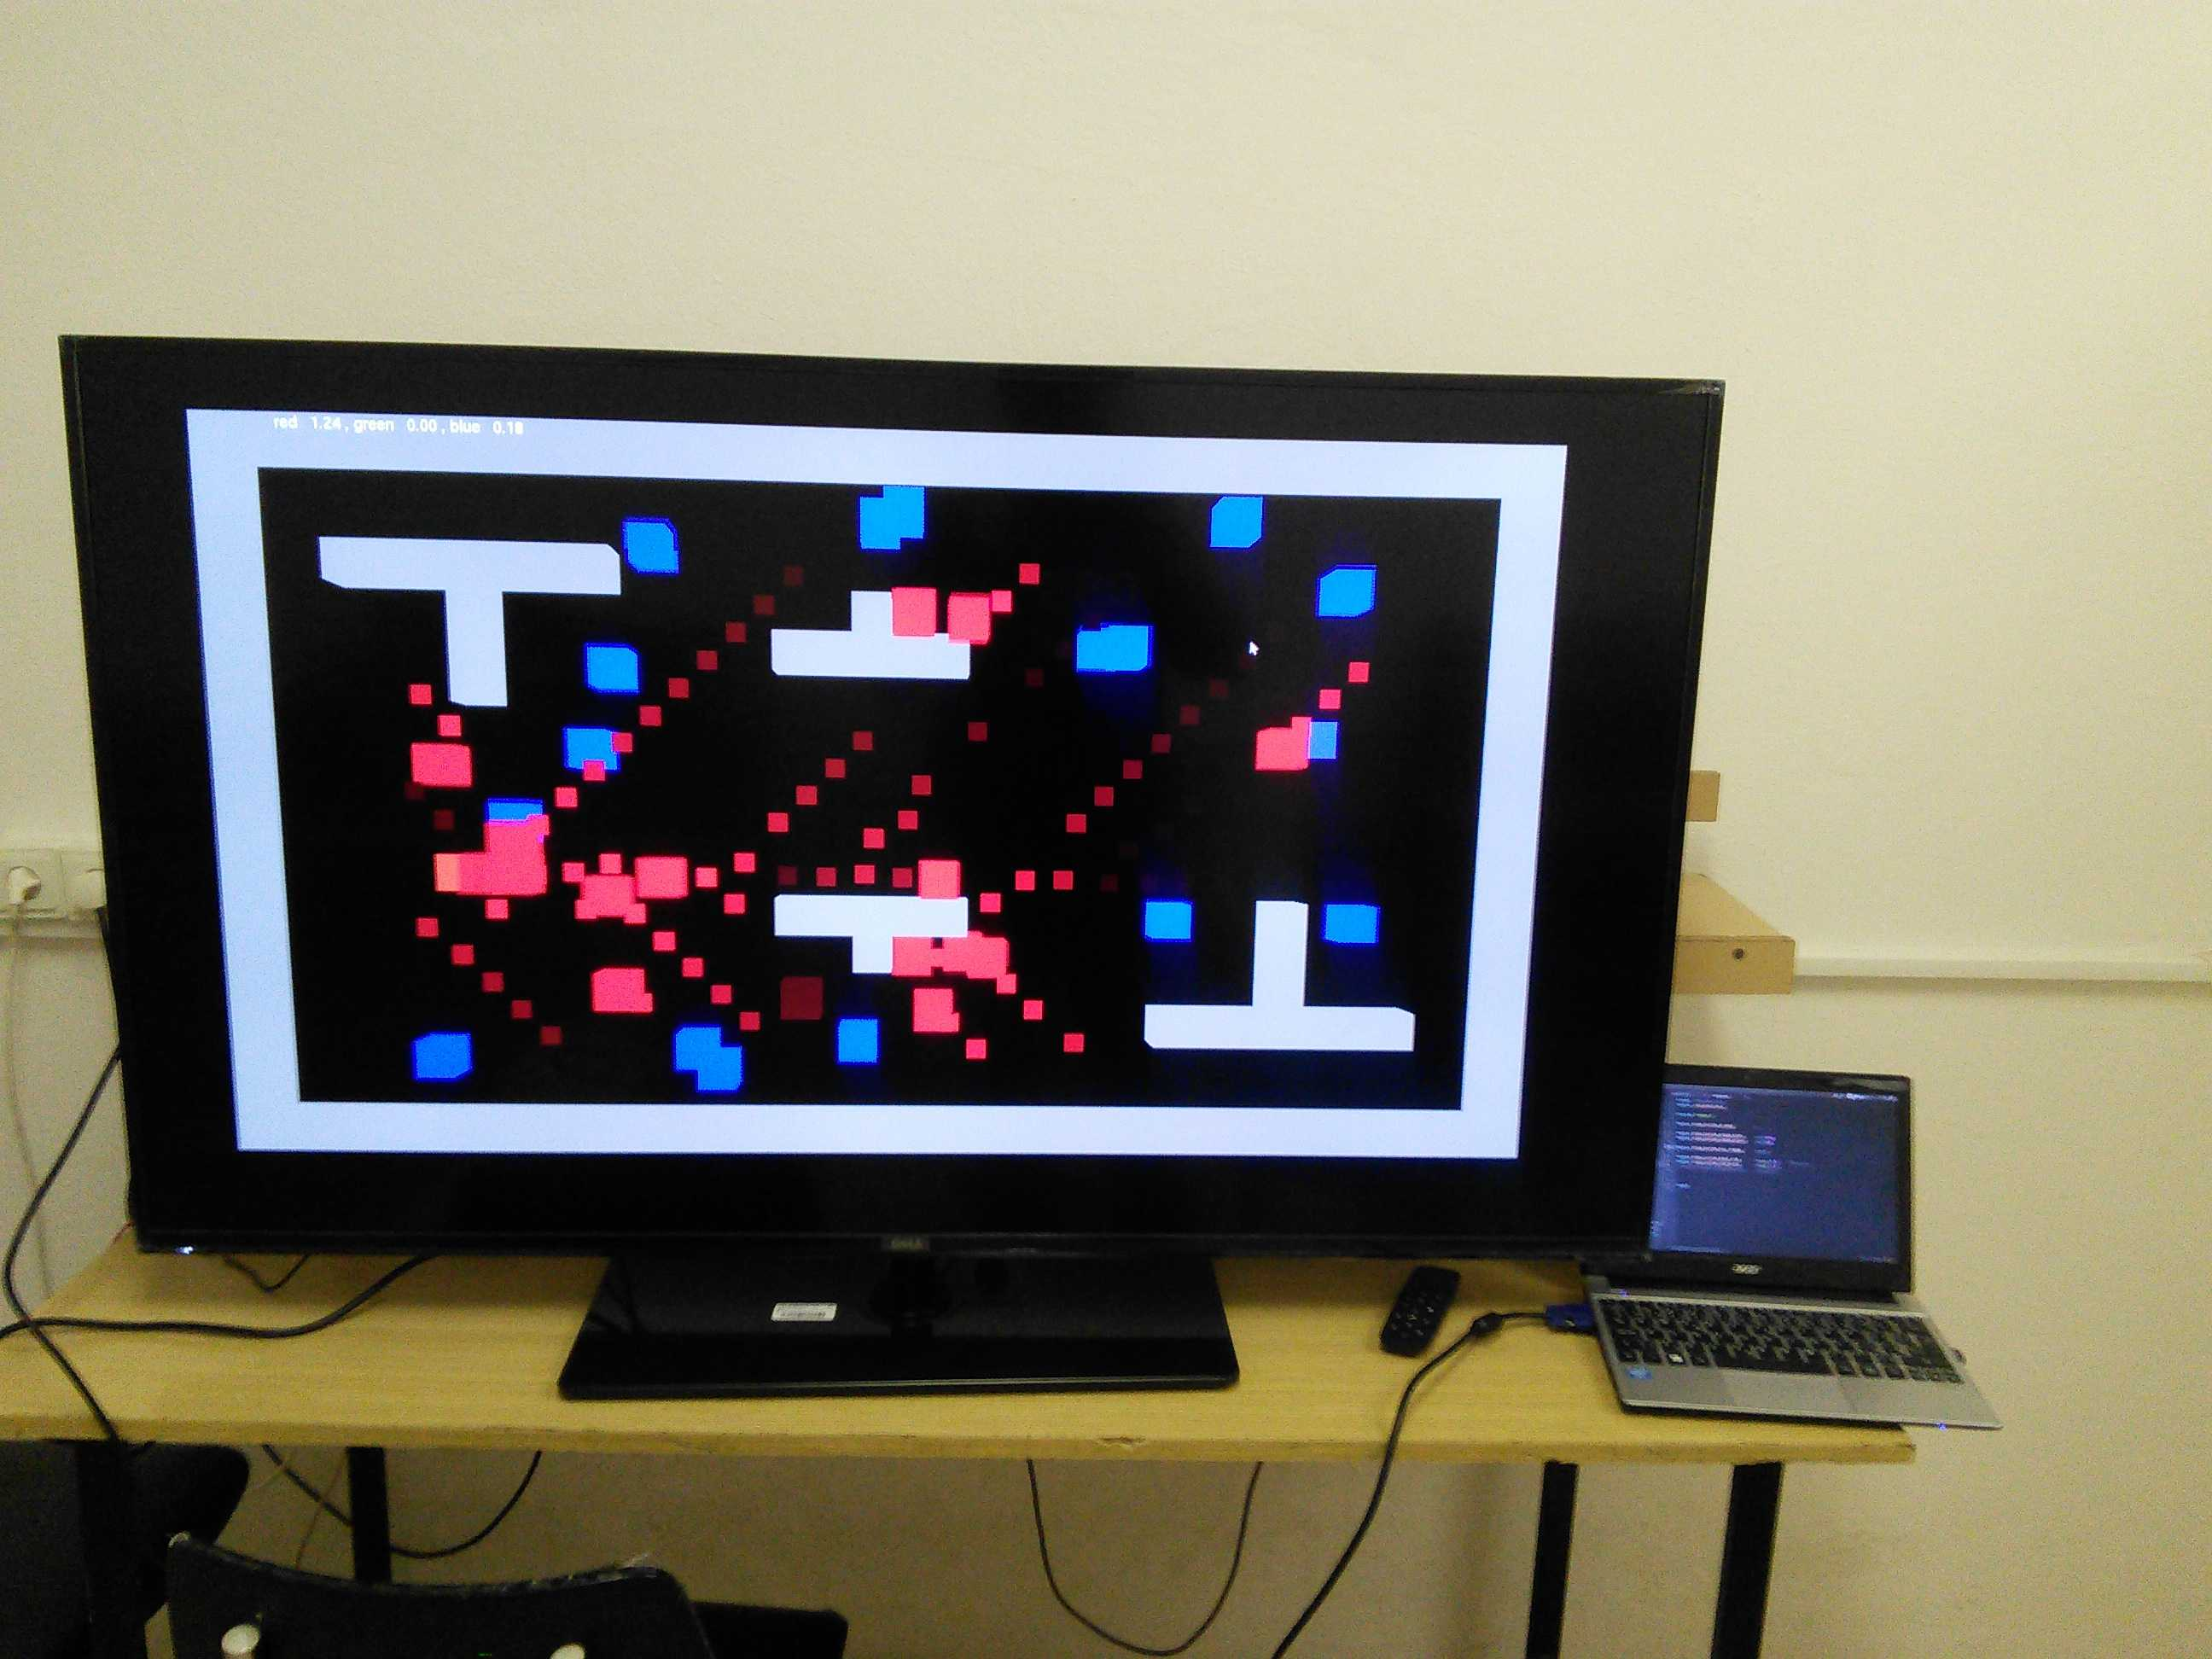
\includegraphics[width=1.0\textwidth]{images/aeris_01.jpg}
\end{center}
\end{minipage}
\end{center}
\end{figure}

\end{frame}


%-------------------------------------------------------------------------------------
\begin{frame}{\bf Súčasný stav projektu}

\begin{figure}[ht]
\begin{center}
\begin{minipage}{0.8\linewidth}
\begin{center}
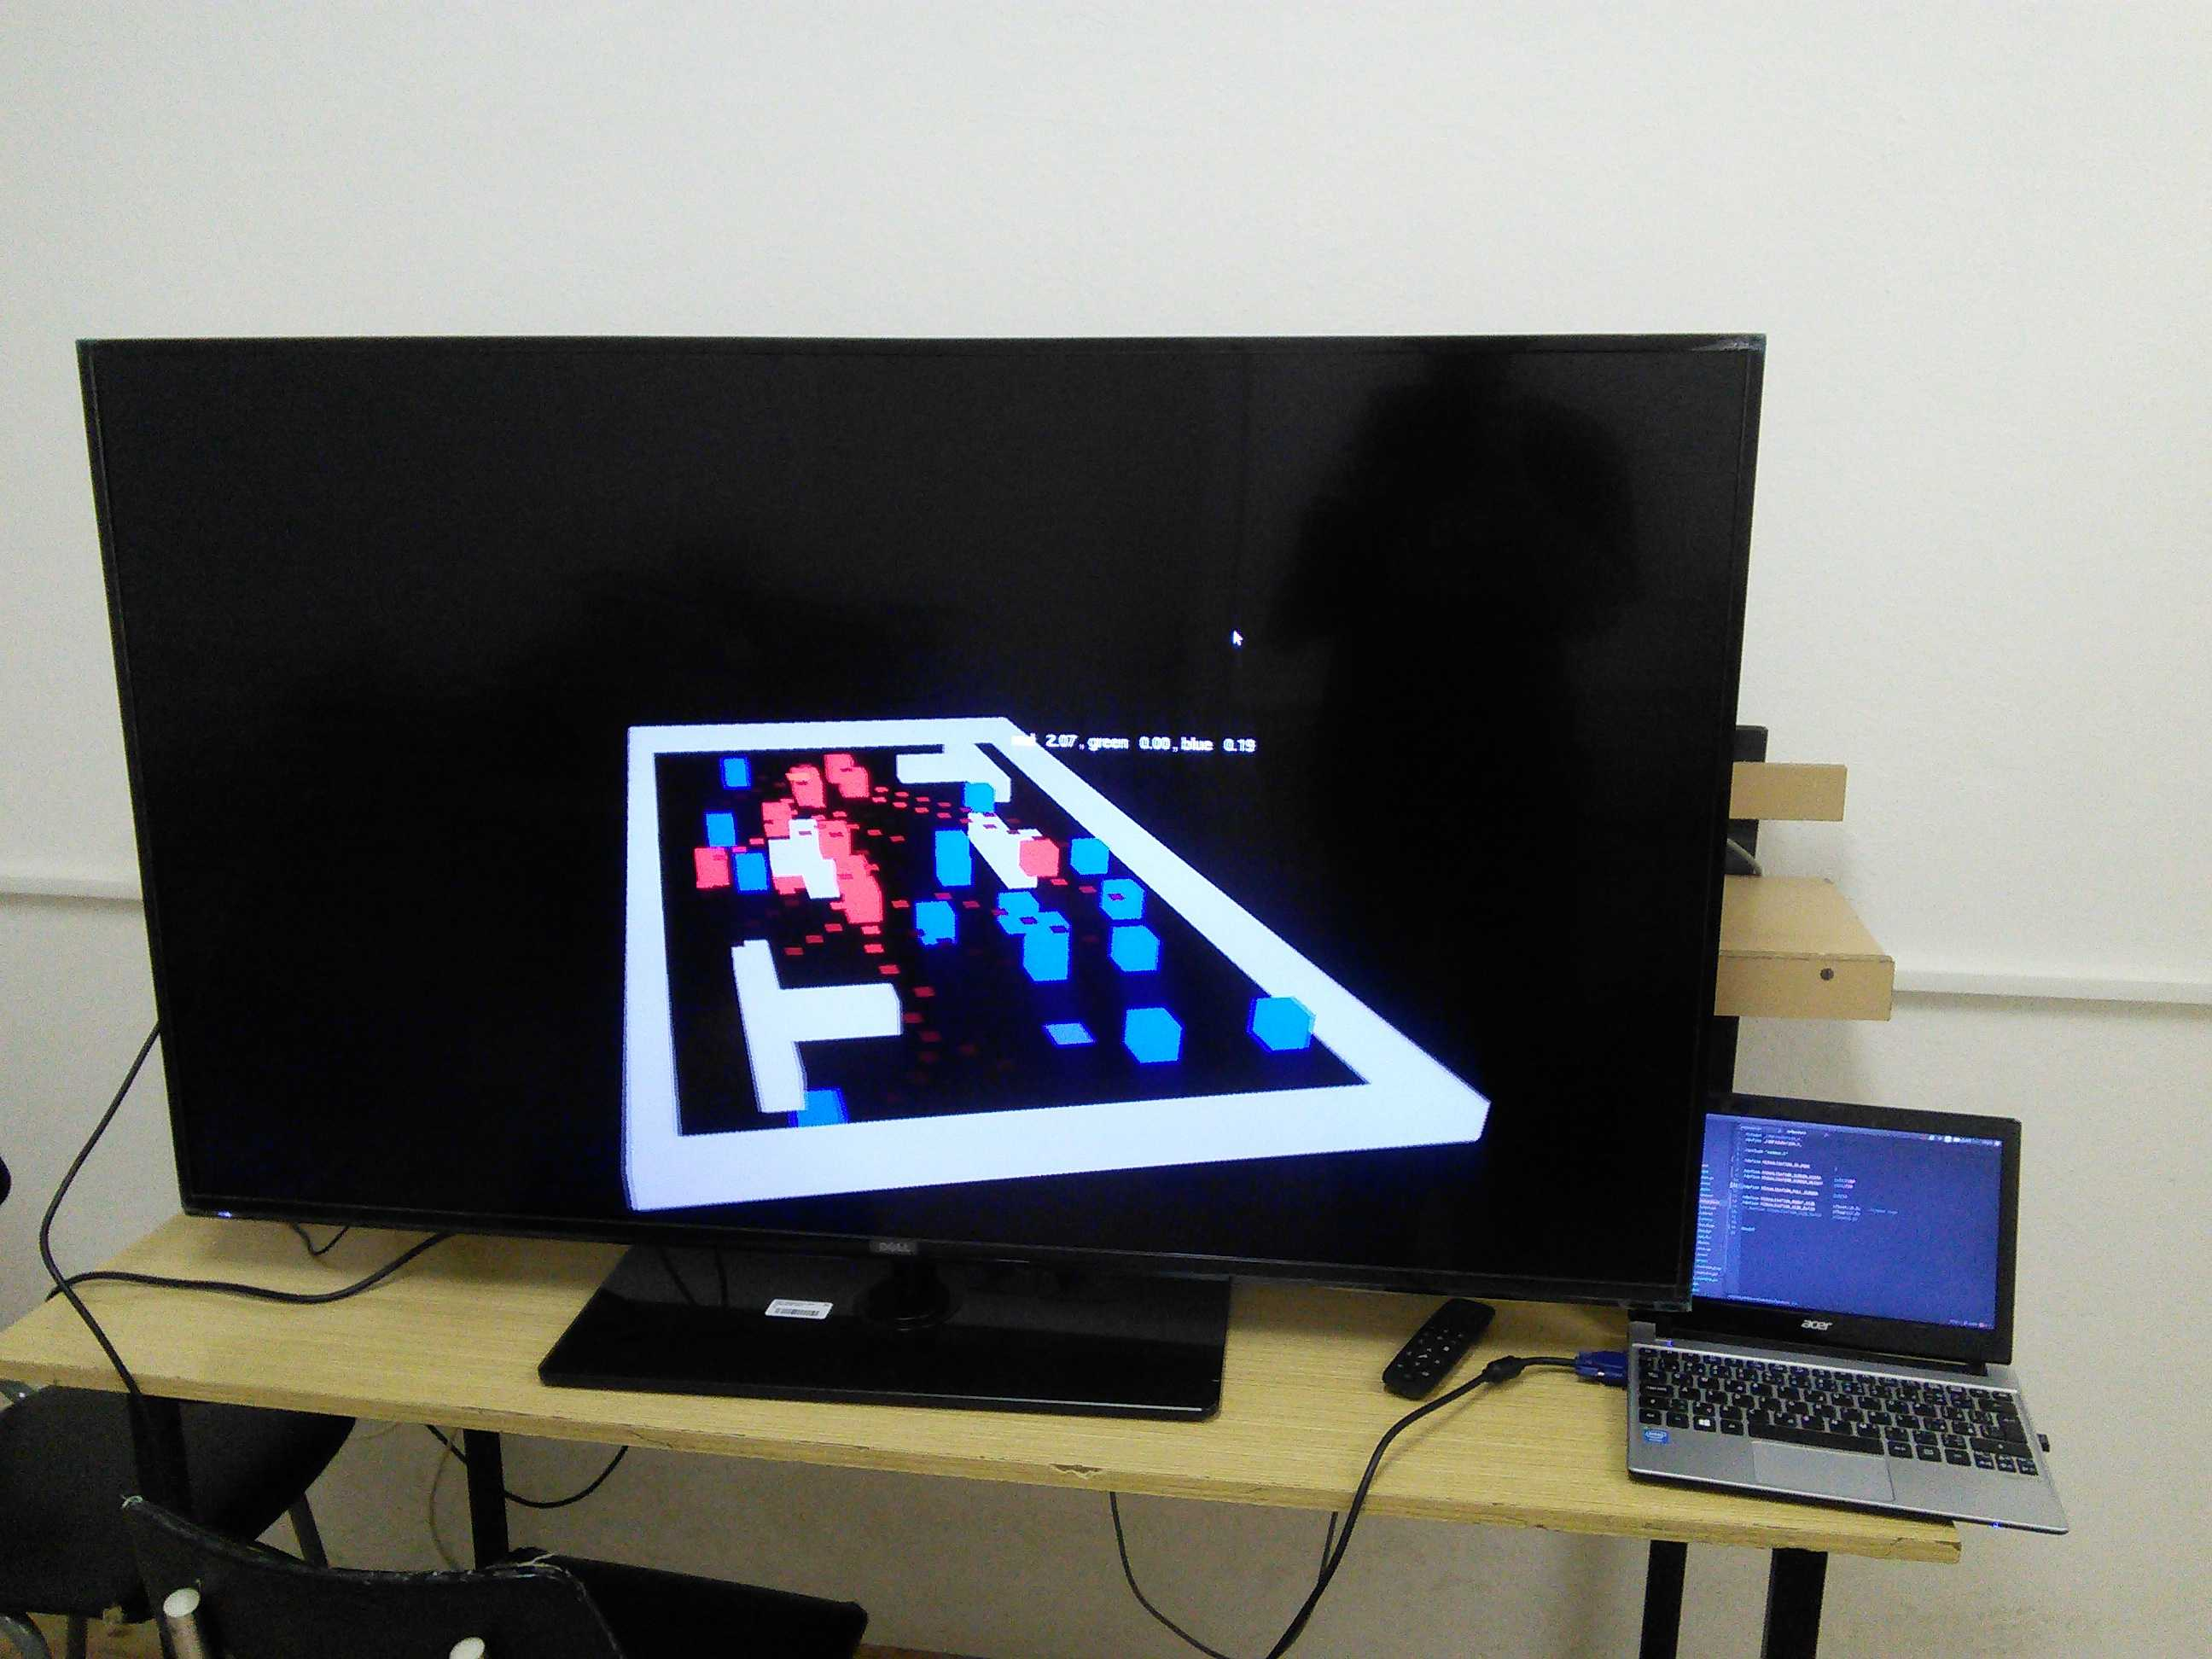
\includegraphics[width=1.0\textwidth]{images/aeris_02.jpg}
\end{center}
\end{minipage}
\end{center}
\end{figure}

\end{frame}


%-------------------------------------------------------------------------------------
\begin{frame}{\bf Súčasný stav}

Software

\begin{itemize}
    \item C++ 11, NASA JPL
    \item OpenGL
    \item Modularita na niekoľkých úrovniach (environment, agent, q\_func, neural\_network, map)
    \end{itemize}


\end{frame}

%-------------------------------------------------------------------------------------
\begin{frame}{\bf Súčasný stav projektu - software}

\begin{enumerate}
    \item common files
    \item map editor
    \item neural network test
    \item q-learning test
    \item virtual robot
        \begin{enumerate}
            \item agent
            \item action
            \item collective\_brain
            \item environment
            \item server
            \item visualisation
        \end{enumerate}
\end{enumerate}

\end{frame}


%-------------------------------------------------------------------------------------
\begin{frame}{\bf Súčasný stav projektu - hardware}

\begin{columns}
	\begin{column}{0.48\textwidth}

	\begin{figure}[ht]
	\begin{center}
	\begin{minipage}{0.9\linewidth}
	\begin{center}
	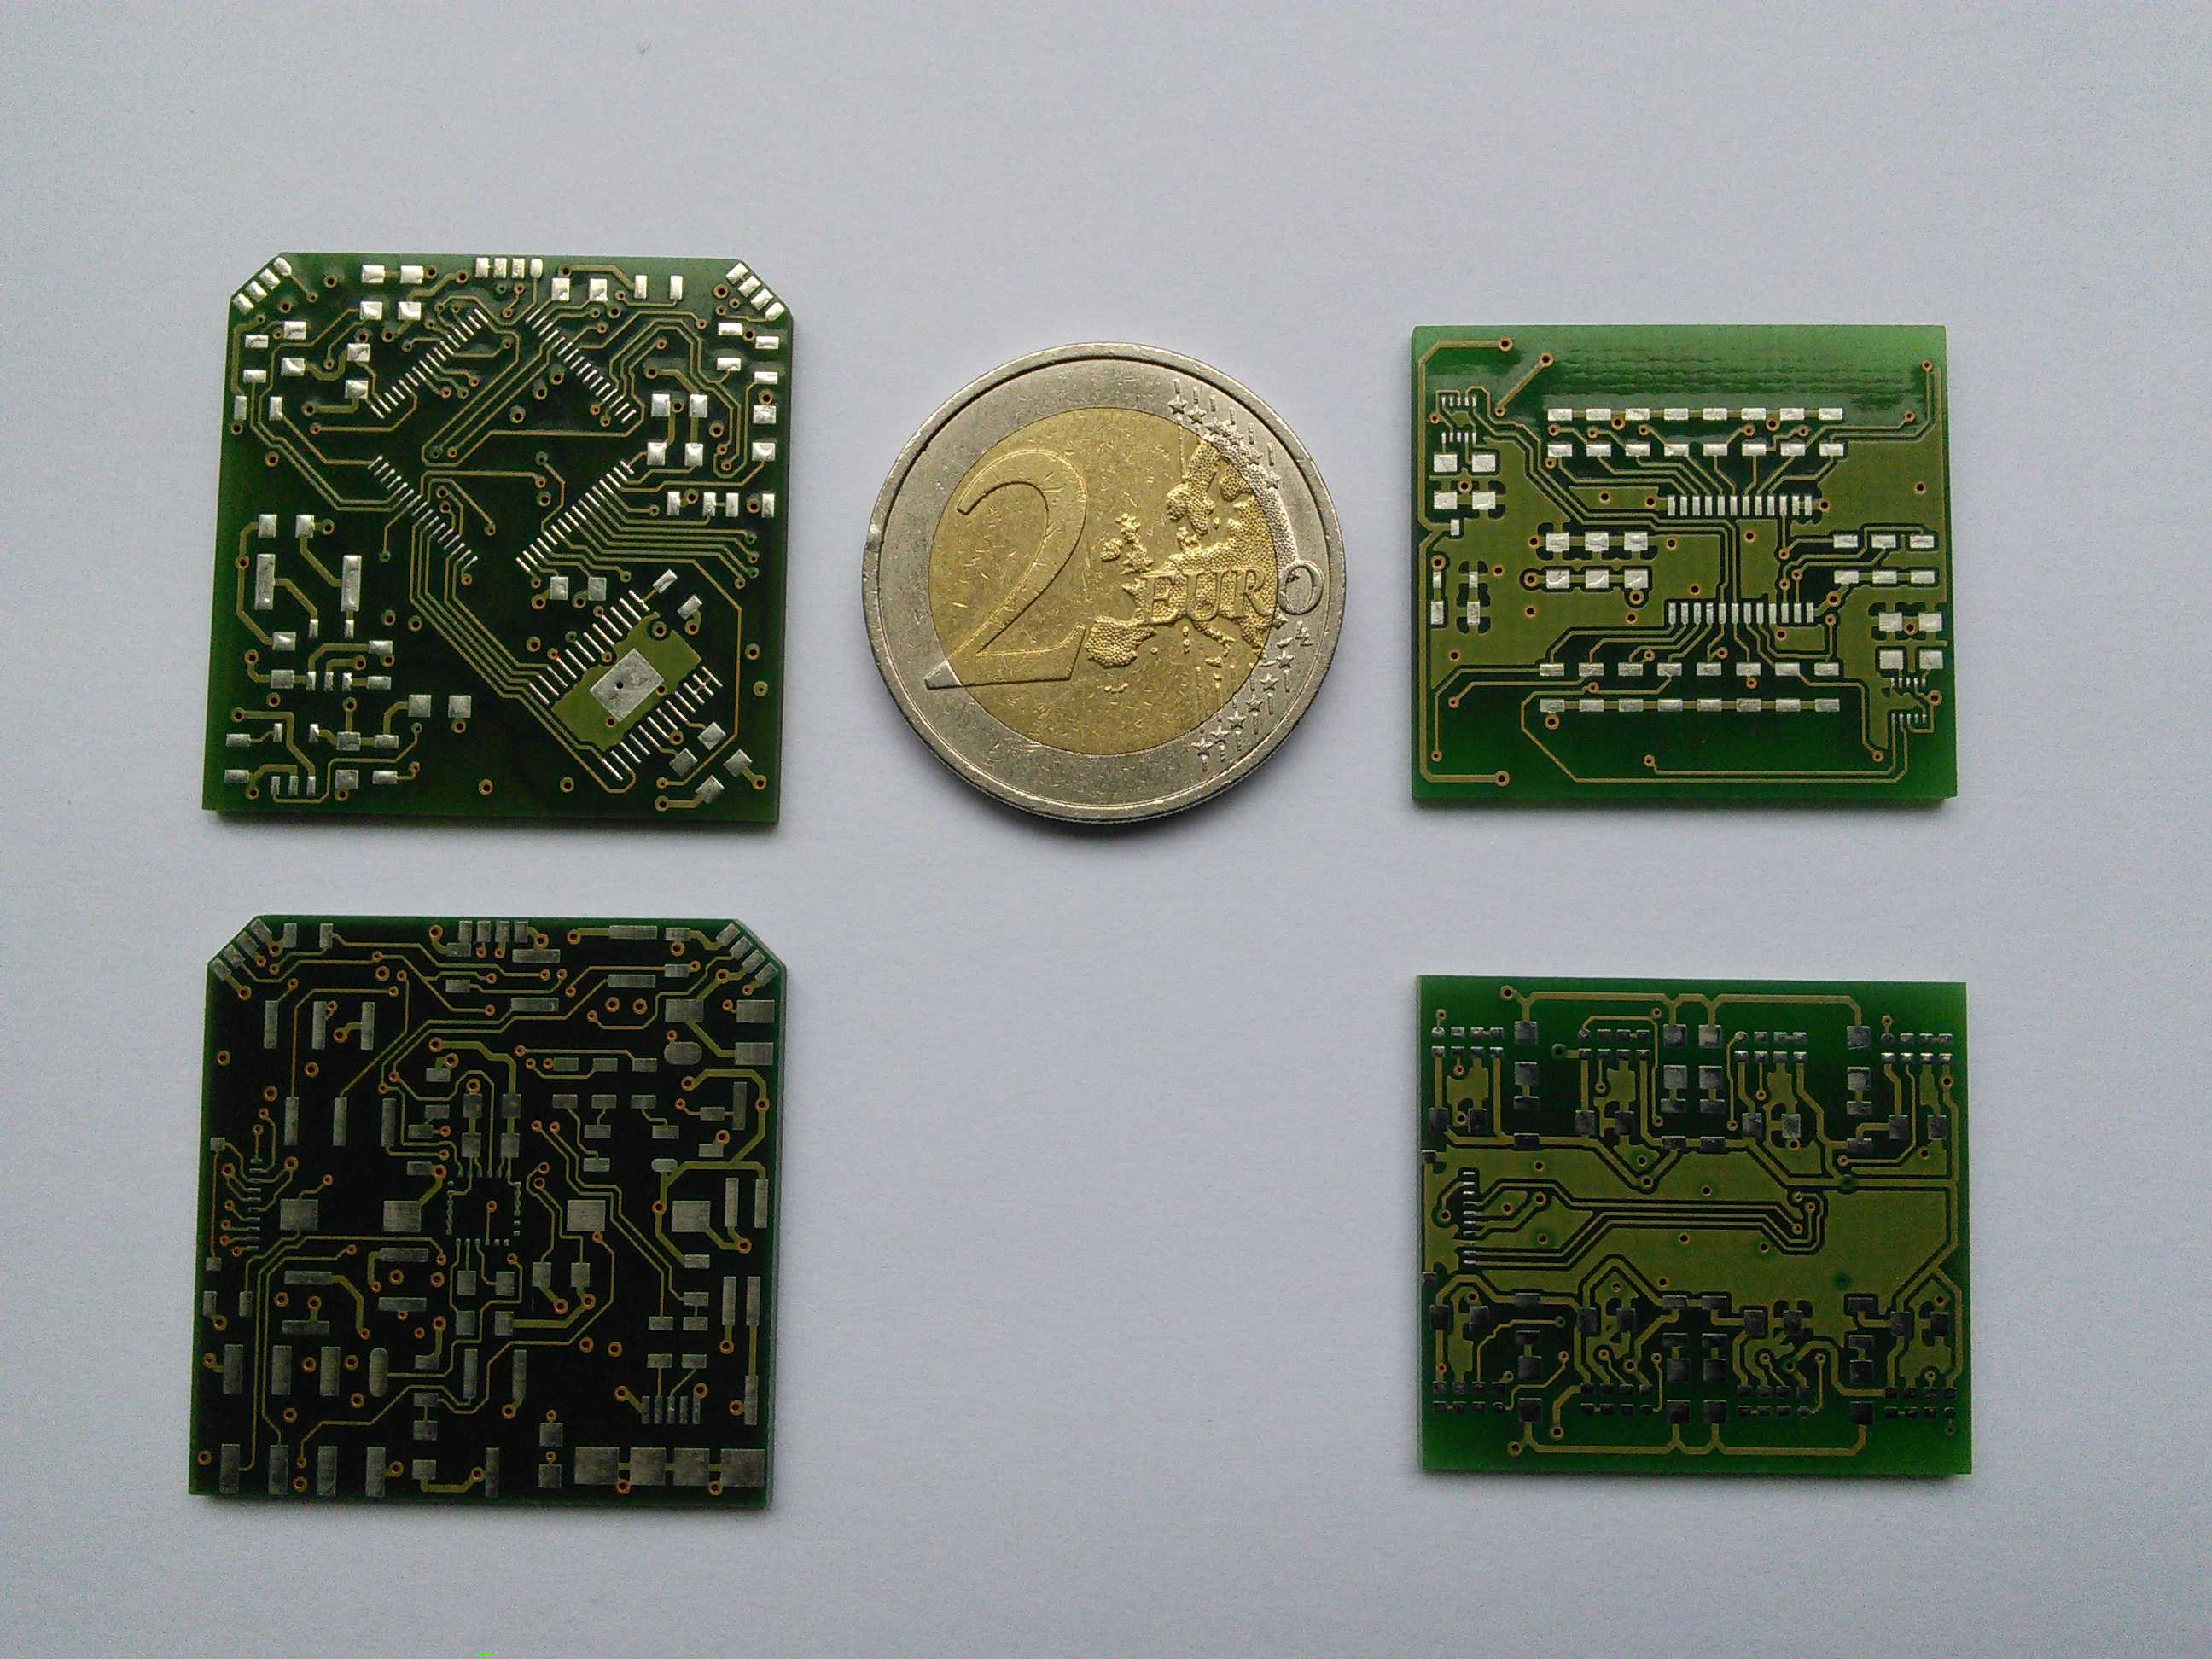
\includegraphics[width=0.9\textwidth]{images/board.jpg}
	\end{center}
	\end{minipage}
	\end{center}
	\end{figure}

	\end{column}
	\begin{column}{0.48\textwidth}
		\begin{enumerate}
            \item ARM Cortex M4F (FPU, oss nastroje), 100MHz, 32bit
            \item 2x motor s prevodovkou
            \item WIFI
            \item USB, I2C
            \item 6x RGB sensor
			\item 3x senzor vzdialenosti
            \item akclerometer, magnetometer, gyroskop
            \item 2x magnetický enkóder
            \item 35mm
		\end{enumerate}
	\end{column}
\end{columns}

\end{frame}

%-------------------------------------------------------------------------------------
\begin{frame}{\bf Očakávané výsledky}

		\begin{enumerate}
            \item lepšie pochopenie procesu rozhodovania
            \item ,,inteligencia'' roja
            \item pochopenie neokortexového stĺpca
            \item riadenie v reálnom čase (10..50ms)
		\end{enumerate}

\end{frame}


%-------------------------------------------------------------------------------------
\begin{frame}{\bf Ďakujem za pozornosť}

\begin{figure}[ht]
\begin{center}
\begin{minipage}{0.4\linewidth}
\begin{center}
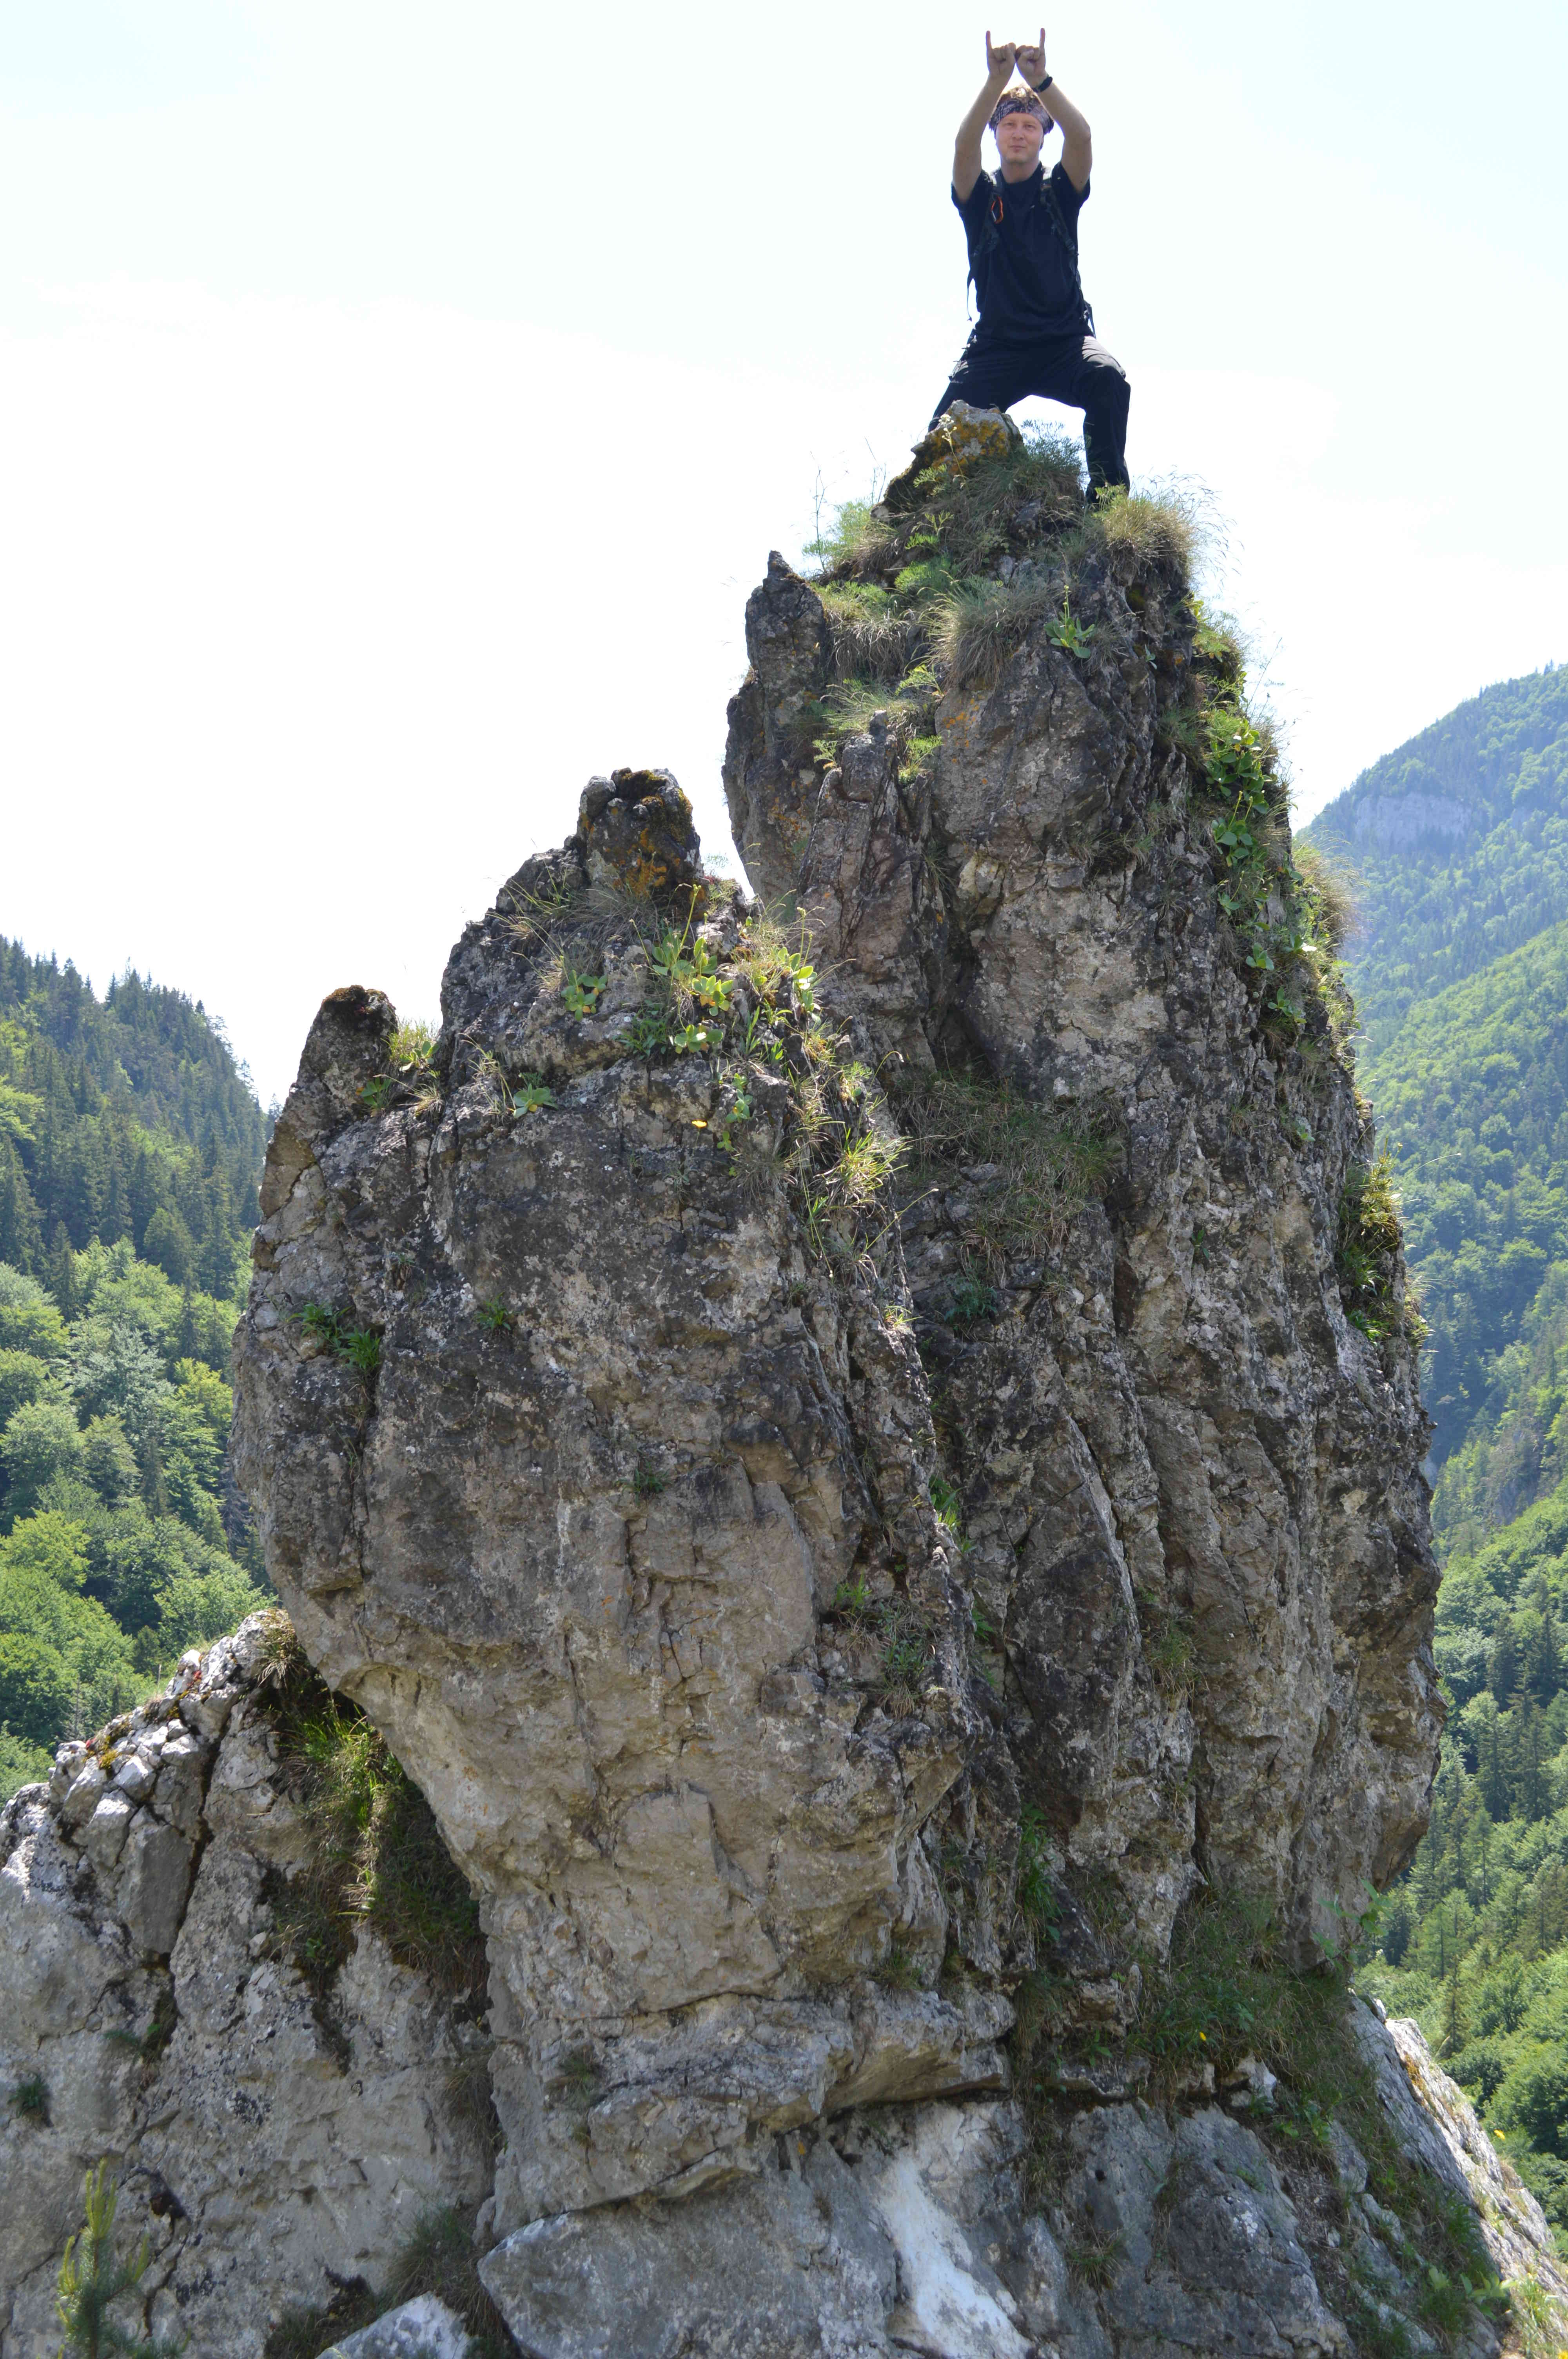
\includegraphics[width=1.0\textwidth]{images/rock.jpg}
\end{center}
\end{minipage}
\end{center}
\end{figure}

\centerline{https://github.com/michalnand/aeris}
\centerline{michal.chovanec@yandex.ru}

\end{frame}

\end{document}
